	\documentclass[
    DIV12,
    cleardouble=plain,
    headings=normal,
    pdftex,
    headexclude,footexclude,
    final
]{scrreprt}


\usepackage[dvipsnames]{xcolor} % for kotlin	
%\usepackage{spreadtab}
\usepackage{xspace}
\usepackage[ngerman]{babel}
\usepackage[utf8]{inputenc}
%\usepackage[T1]{fontenc}
\usepackage[pdftex]{graphicx}
\usepackage[bookmarks]{hyperref}
\usepackage{scrpage2}
\usepackage{longtable}
\usepackage{caption}
\usepackage{pgfplots}
\usepackage{float}
%\usepackage{xcolor}
\usepackage{colortbl}
\usepackage{tabularx}
\usepackage{multirow} % tabelle
\usepackage{listings} % code aus datei einbinden
\usepackage{scrhack}
\usepackage{comment}




% word wrap with a red arrow
\lstset{
  basicstyle=\ttfamily,
  columns=fullflexible,
  frame=single,
  breaklines=true,
  postbreak=\mbox{\textcolor{red}{$\hookrightarrow$}\space},
}

\graphicspath{{./}{./images/}}


% kotlin syntax highlighting
\lstdefinelanguage{Kotlin}{
  keywords={package, as, typealias, this, super, val, var, fun, for, null, true, false, is, in, throw, return, break, continue, object, if, try, else, while, do, when, yield, typeof, yield, typeof, class, interface, enum, object, override, public, private, get, set, import, abstract, },
  keywordstyle=\color{NavyBlue}\bfseries,
  ndkeywords={@Deprecated, Iterable, Int, Integer, Float, Double, String, Runnable, dynamic},
  ndkeywordstyle=\color{BurntOrange}\bfseries,
  emph={println, return@, forEach,},
  emphstyle={\color{OrangeRed}},
  identifierstyle=\color{black},
  sensitive=true,
  commentstyle=\color{gray}\ttfamily,
  comment=[l]{//},
  morecomment=[s]{/*}{*/},
  stringstyle=\color{ForestGreen}\ttfamily,
  morestring=[b]",
  morestring=[s]{"""*}{*"""},
}



% word wrap with a red arrow
\lstset{
  basicstyle=\ttfamily,
  columns=fullflexible,
  frame=single,
  breaklines=true,
  postbreak=\mbox{\textcolor{red}{$\hookrightarrow$}\space},
}

% #################################################################

\hyphenation{Cha-otn-gsch-werl}
\setlength\headheight{1.75cm}


\ihead{\small{Android Food Tracking App in Kotlin}}
\chead{}
\ohead{
\includegraphics[height=0.05\textheight]{fh_logo}}
\ifoot{\small{Smartphone Programming III}}
\ofoot{\small{Johannes Franz \& Normen Krug}}
\pagestyle{scrheadings}









\setcounter{secnumdepth}{5}
\setcounter{tocdepth}{5}
\renewcommand{\arraystretch}{1}

\parskip0.5\baselineskip plus 0.125\baselineskip minus 0.25\baselineskip
\parindent0em

%\automark[section]{chapter}

\titlehead{\begin{center}
\includegraphics[width=5cm]{fh_logo}\end{center}}
 \title{
  Entwicklung einer Android Food Tracking App \\[1em]
  in der Programmiersprache Kotlin  
}
\publishers{Vorgelegt bei Prof. Dr. Michael Stepping}

\author{Johannes Franz \& Normen Krug}


\date{Wintersemester 2017/2018}


\begin{document}
\maketitle


\pagenumbering{roman}

\tableofcontents

%\listoftables

\newpage
\pagenumbering{arabic}


\chapter{Einleitung}
Ziel ist es eine Open Source App zu entwickeln, die einen Rückschluss von sich zugenommener Nahrung auf Symptome zu ermöglichen. Dabei helfen die in der App eingetragenen Datenpunkte und Fotos diese z.B. mit einer allergischen Reaktion zu verknüpfen.
Zielgruppe sind Menschen, die wegen Erkrankungen aus ihren zu sich zugenommenen Speisen und Getränken Rückschlüsse auf ihr Wohlbefinden treffen wollen, um zukünftig solche Speisen zu meiden.


\newpage

\chapter{Motivation}
Durch eigenen Bedarf motiviert entstand die Idee zu dieser App. Um aus wiederkehrenden Mahlzeiten eine Unverträglichkeit abzuleiten, stellt die App entsprechende Funktionen bereit.
Bei dieser Arbeit war außerdem das Ziel möglichst viele neue Technologien zu verwenden. So wurde bei allen Möglichkeiten der schwierigere Weg gewählt, der jedoch zu neuen Erkenntnissen führte.\\
Beispiele dafür sind:\\
Kotlin, LaTeX, InAPp-SQLite,Dagger, Room, Recycler View, Model View Presenter, Spinner Menu in der Toolbar


\chapter{Kotlin als Programmiersprache}
Für die App wurde die Programmiersprache Kotlin verwendet, welche auf der Google IO im Mai 2017 als offizielle Sprache für Android eingeführt wurde. Kotlin hat einen besser lesbaren Syntax als Java. Wie bei Java wird auch bei Kotlin der Bytecode für die Java Virtual Machine übersetzt. Insgesamt ist Kotlin der Programmiersprache Swift 3 bzw 4 syntaktisch sehr nahe, was den Umgang als Entwickler mobiler Anwendungen zusätzlich erleichtert. Die Entscheidung dieses Sprache zu wählen war wieder davon getrieben etwas neues auszuprobieren.\\

Kotlin Code Beispiel:
\lstinputlisting[language=Kotlin]{content/Kotlin_example.kt}

\newpage

\chapter{Entwurfsphase}
In der Entwurfsphase wurde keine Zeit verschwendet und somit wurde der Fokus auf Handskizzen gelegt. Der Zwischenschritt diese Skizzen in einem professionellen Entwurf nachzubauen sparte Zeit, so dass sich direkt mit der Programmierung beschäftigt werden konnte.



\section{Main Screen}
\begin{figure}[H]
	\centering
  \frame{ 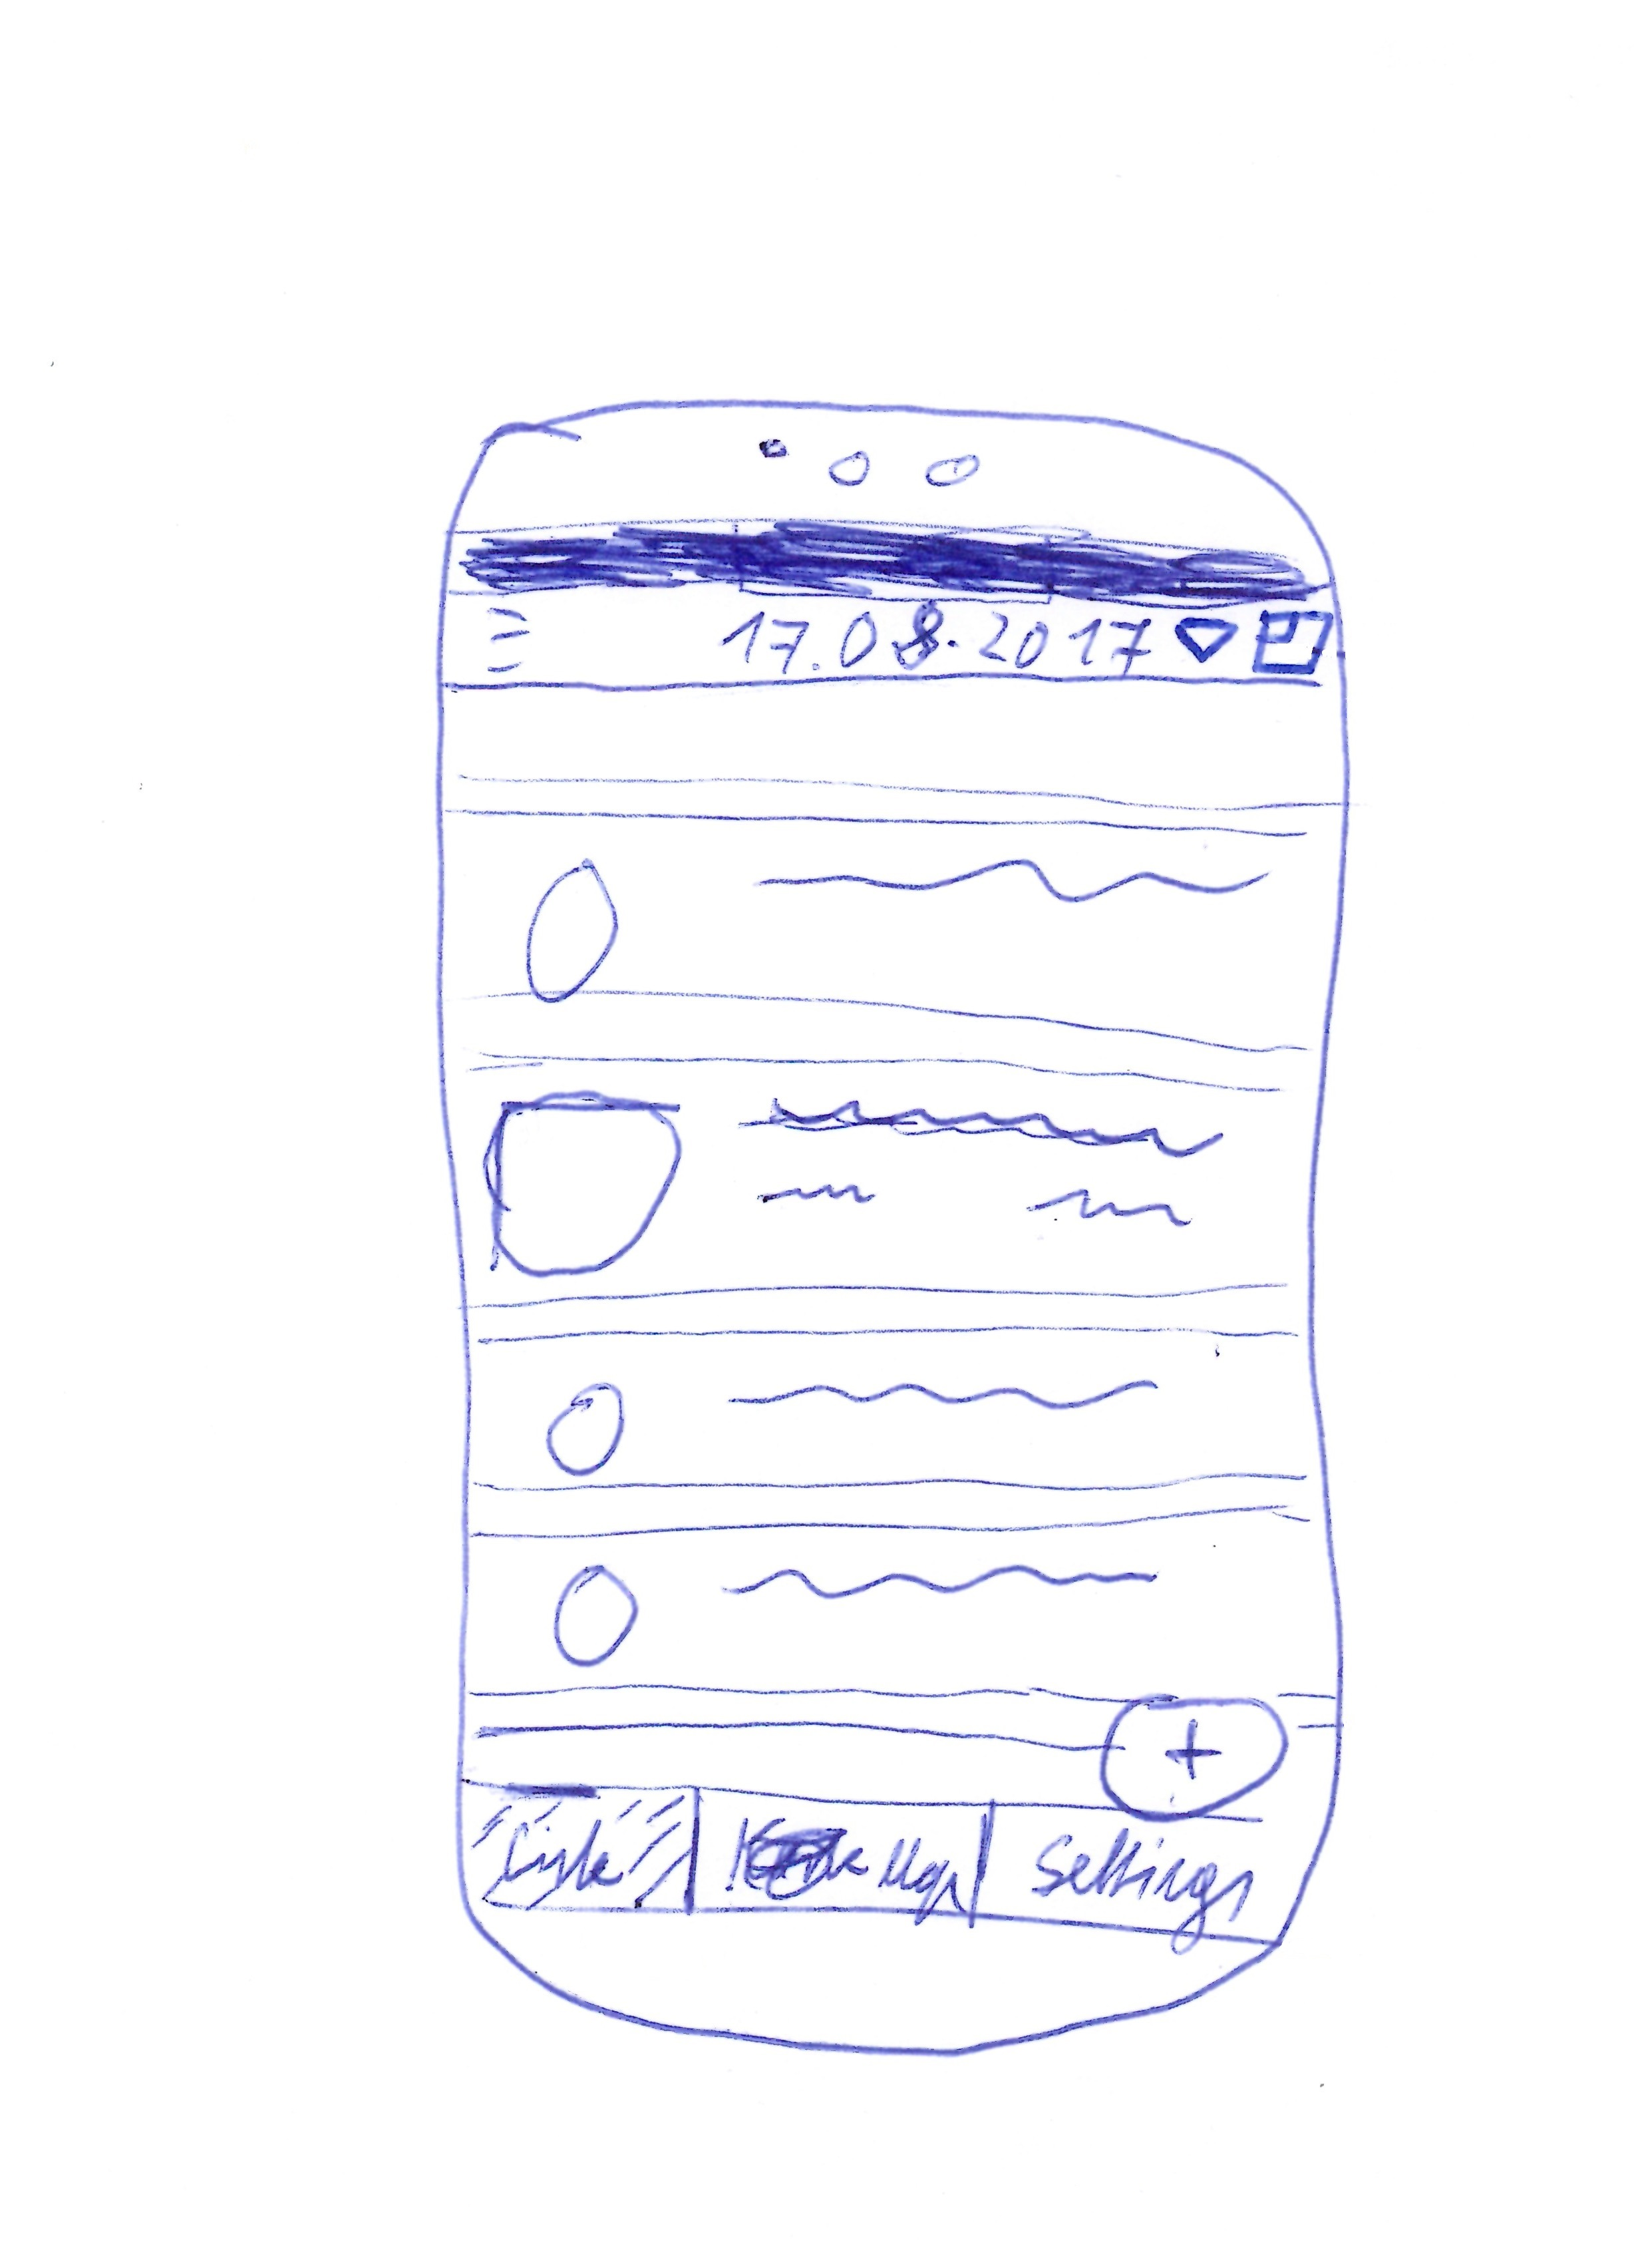
\includegraphics[scale=0.7]{main} }
	\caption{Main Screen}
	\label{main}
\end{figure}


\section{Hinzufügen eines Eintrags}
\begin{figure}[H]
	\centering
  \frame{ 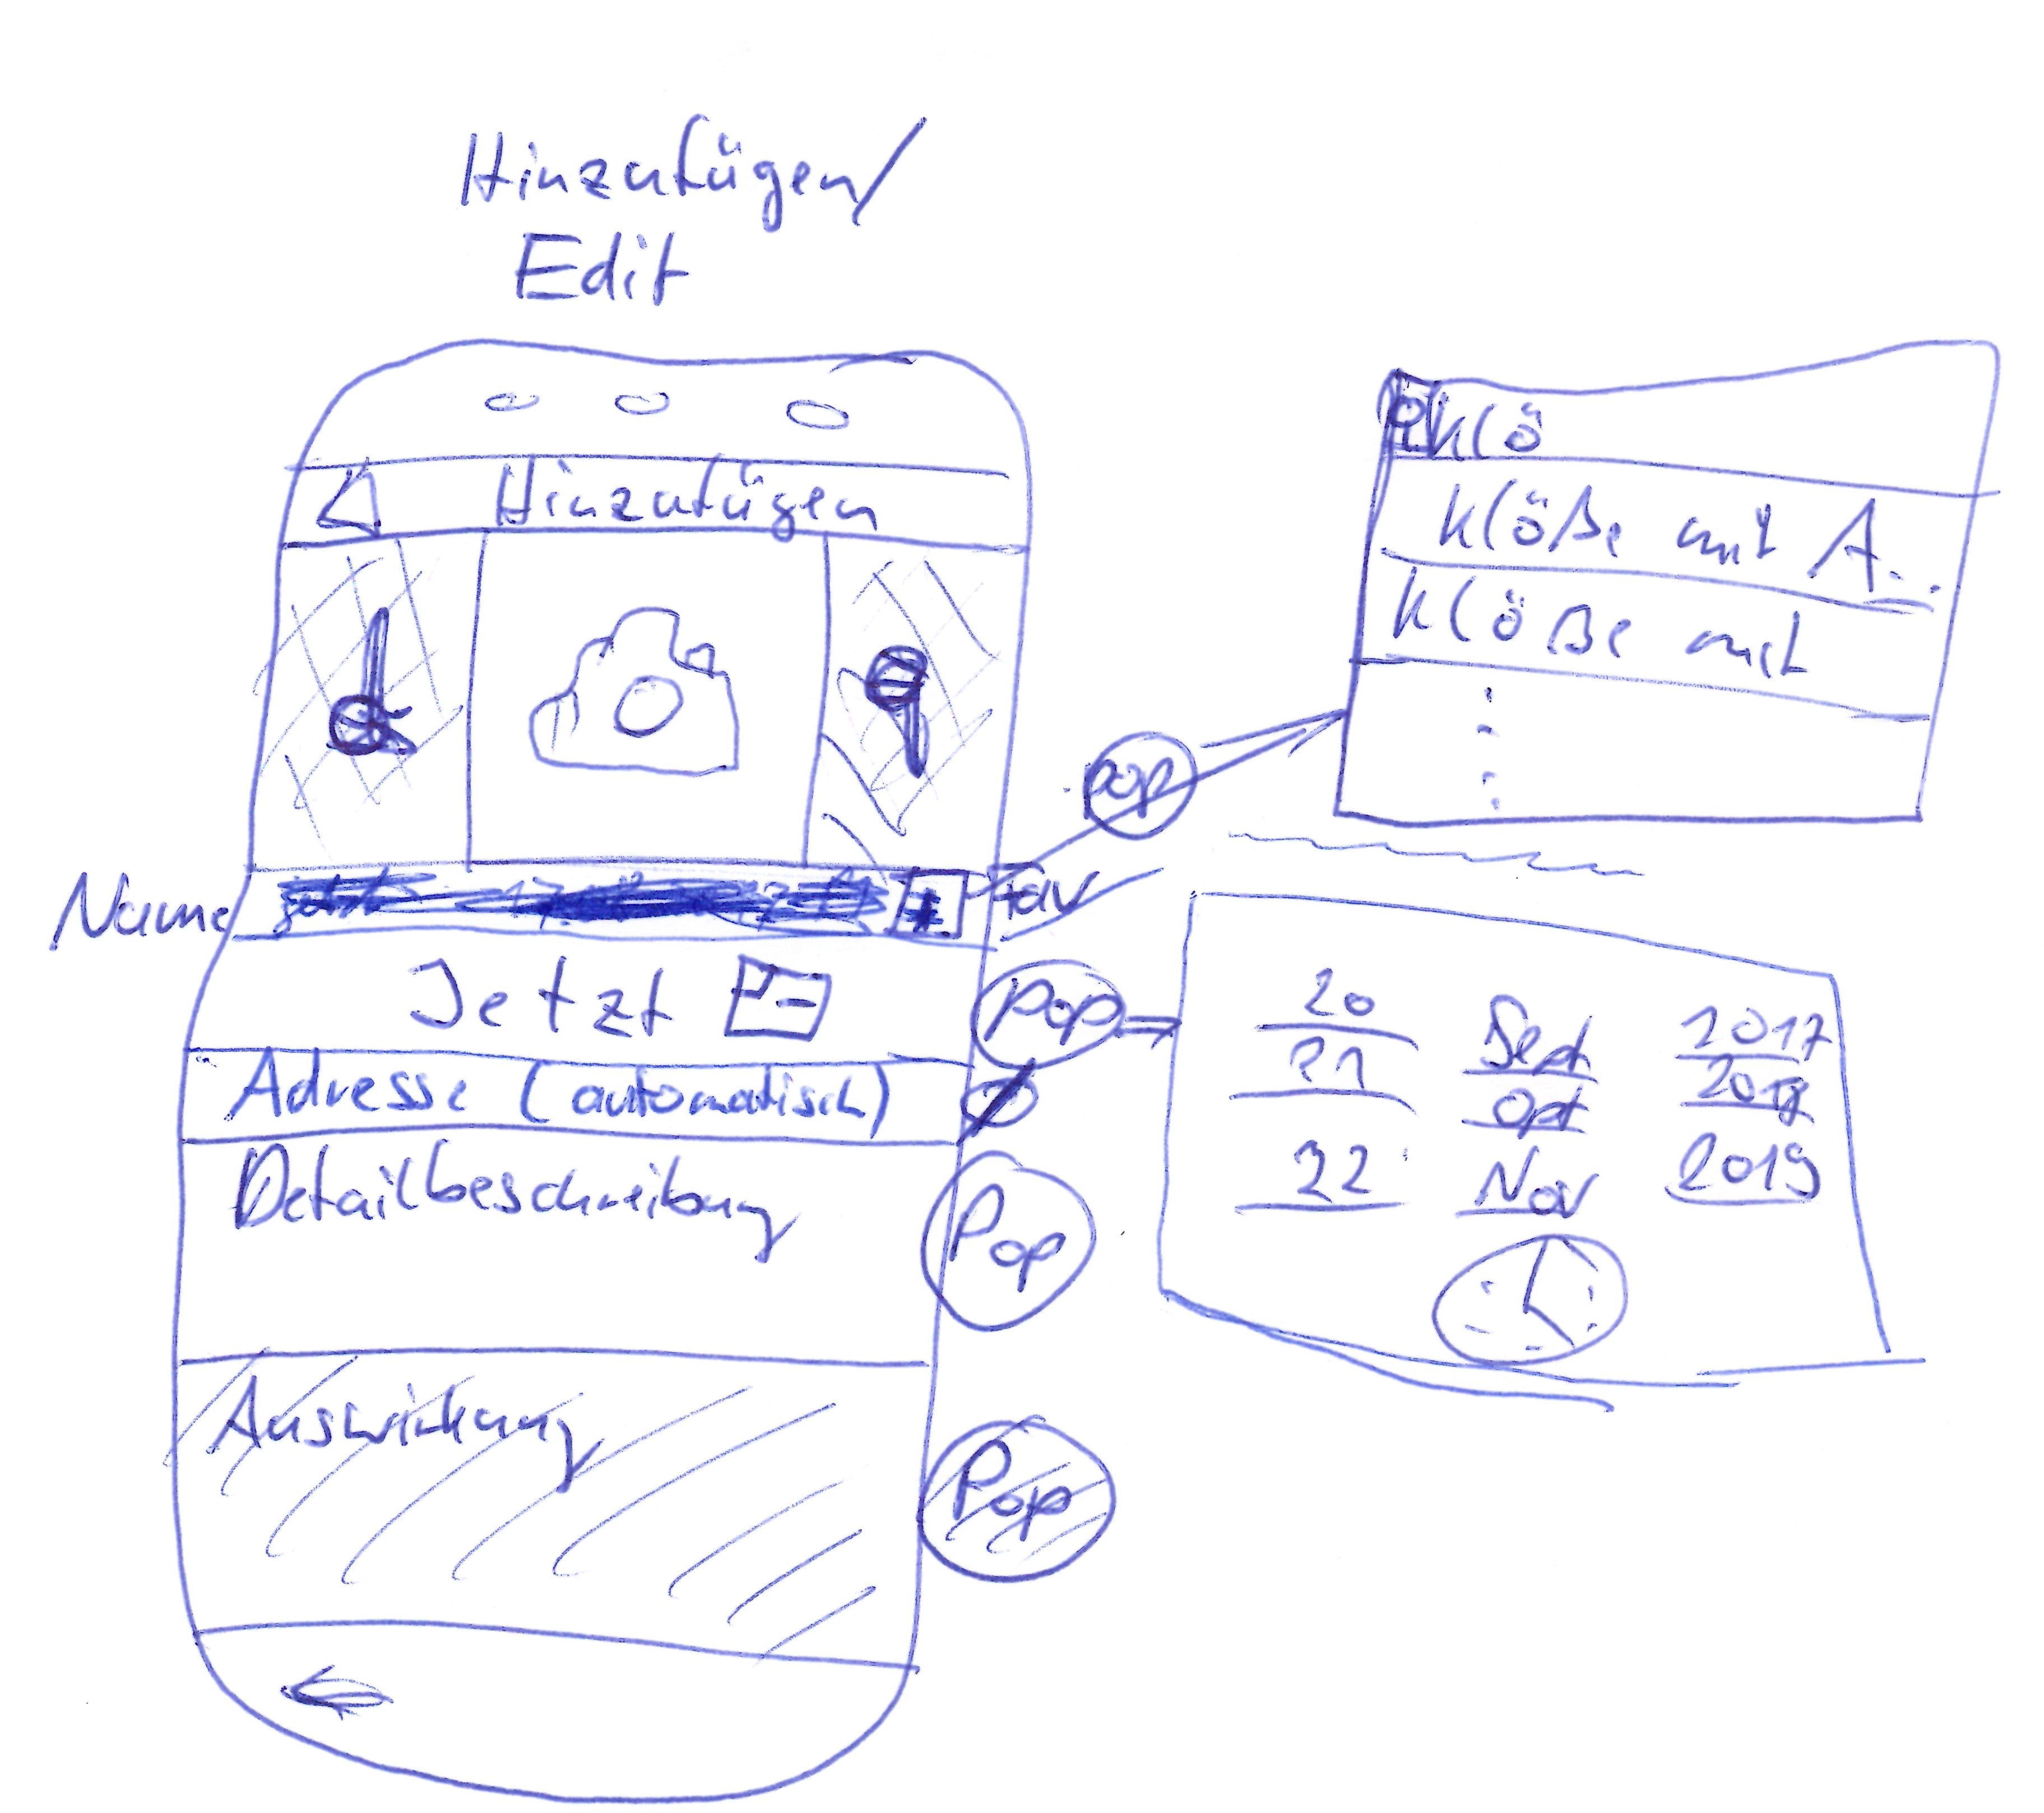
\includegraphics[scale=0.7]{add_entwurf} }
	\caption{Hinzufügen eines Eintrags}
	\label{add_entwurf}
\end{figure}


\section{Popover im Main Screen}
\begin{figure}[H]
	\centering
  \frame{ 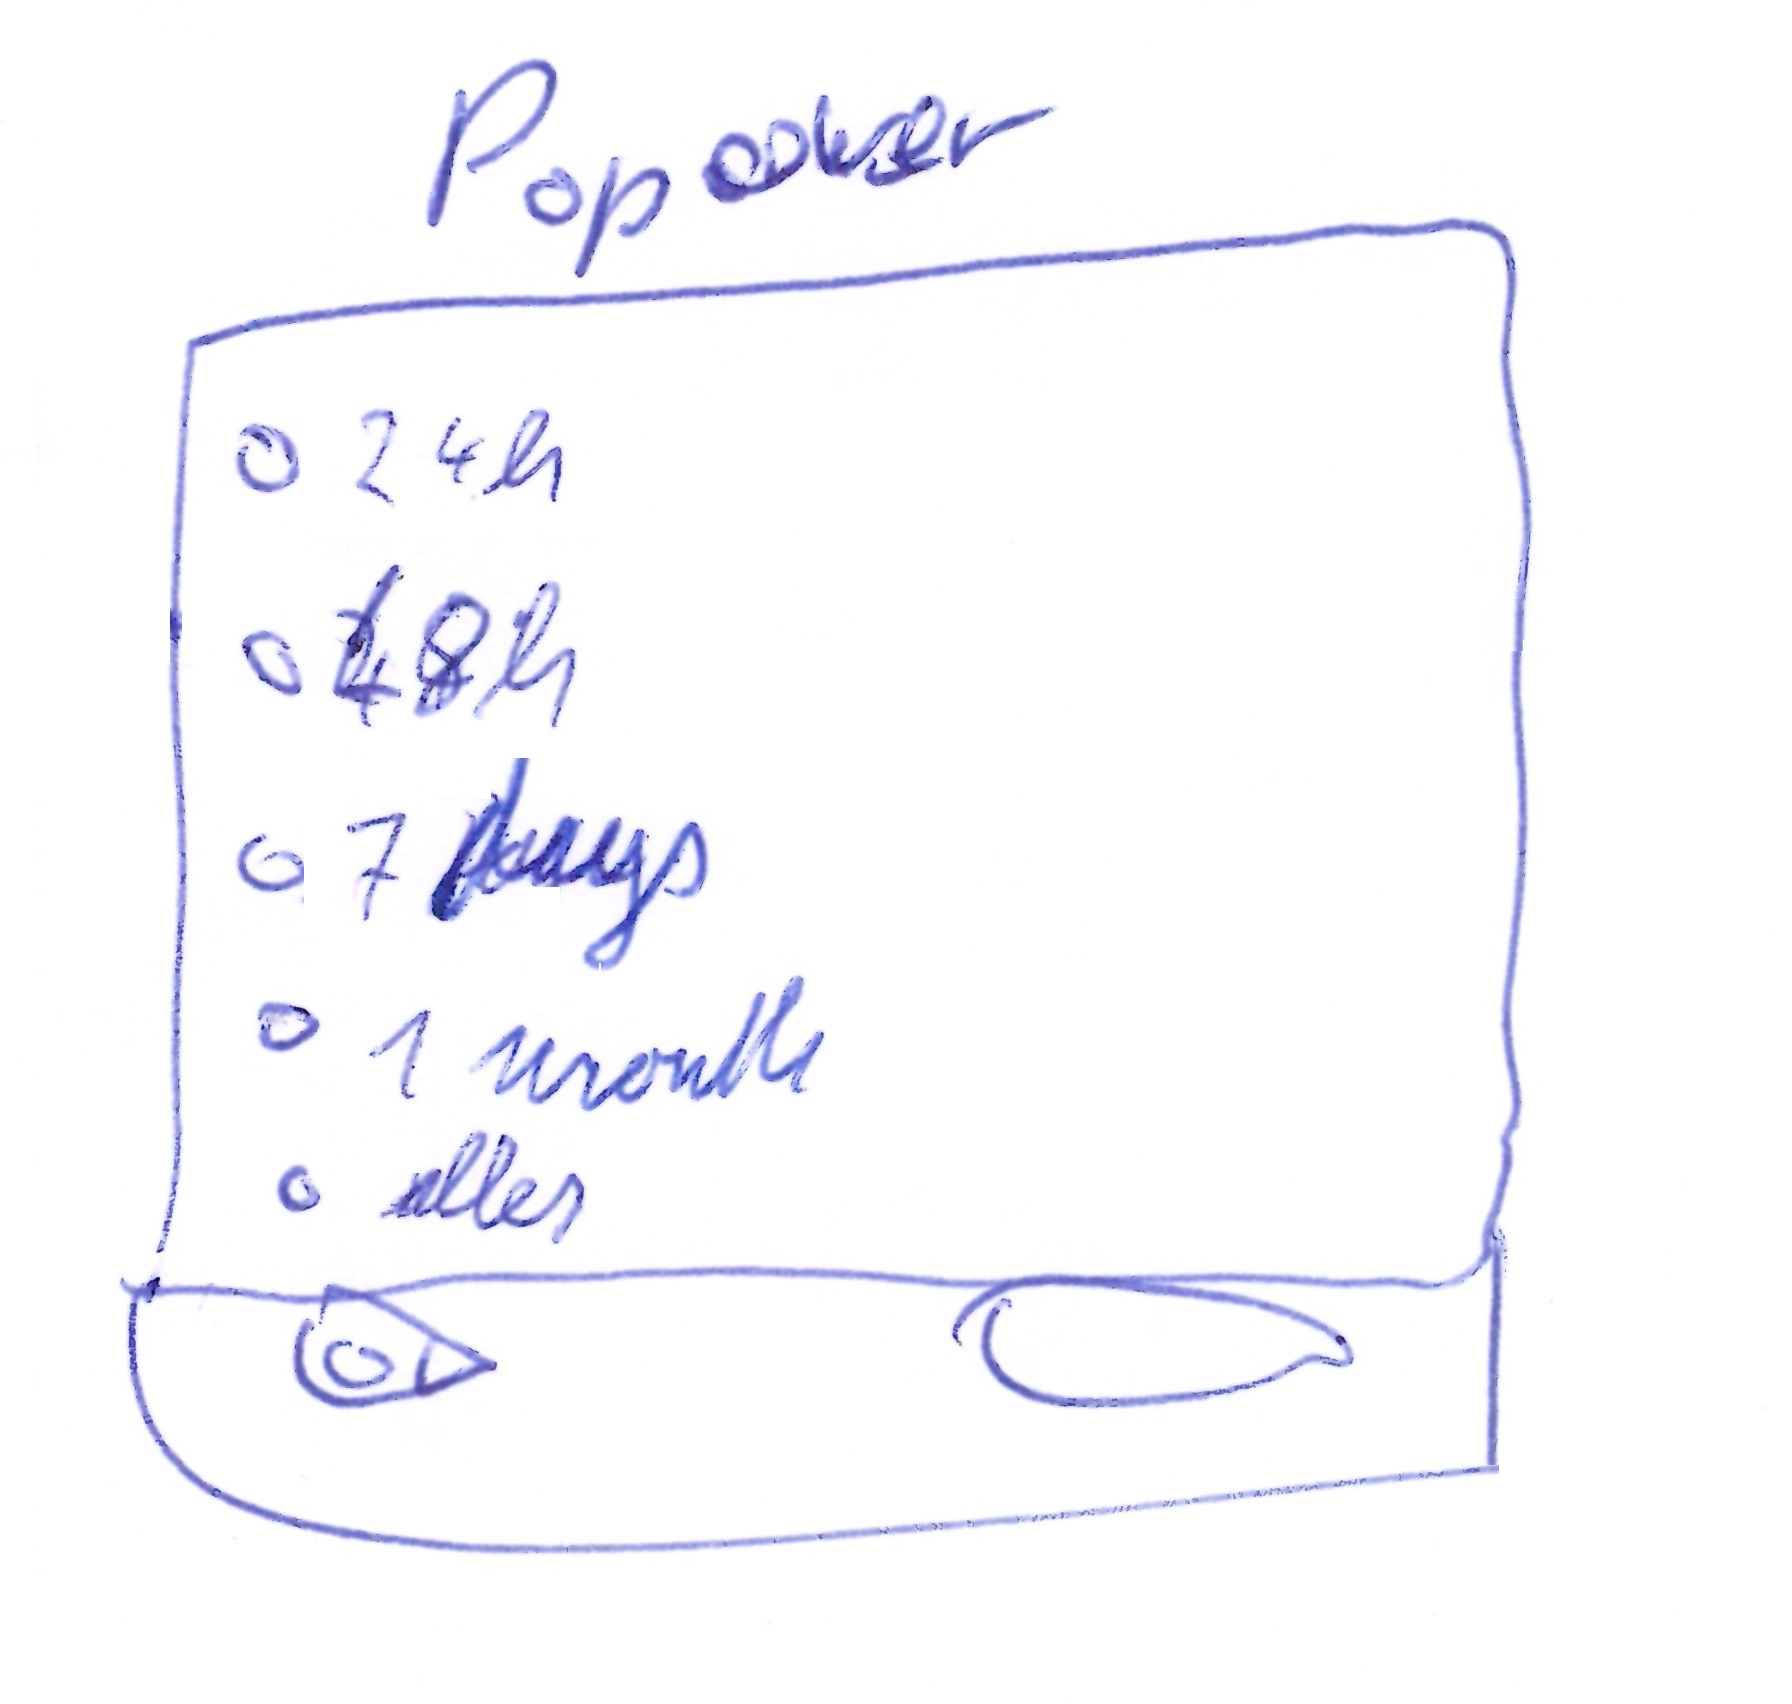
\includegraphics[scale=0.7]{popover} }
	\caption{Popover Screen}
	\label{popover}
\end{figure}


\section{Settings}
\begin{figure}[H]
	\centering
  \frame{ 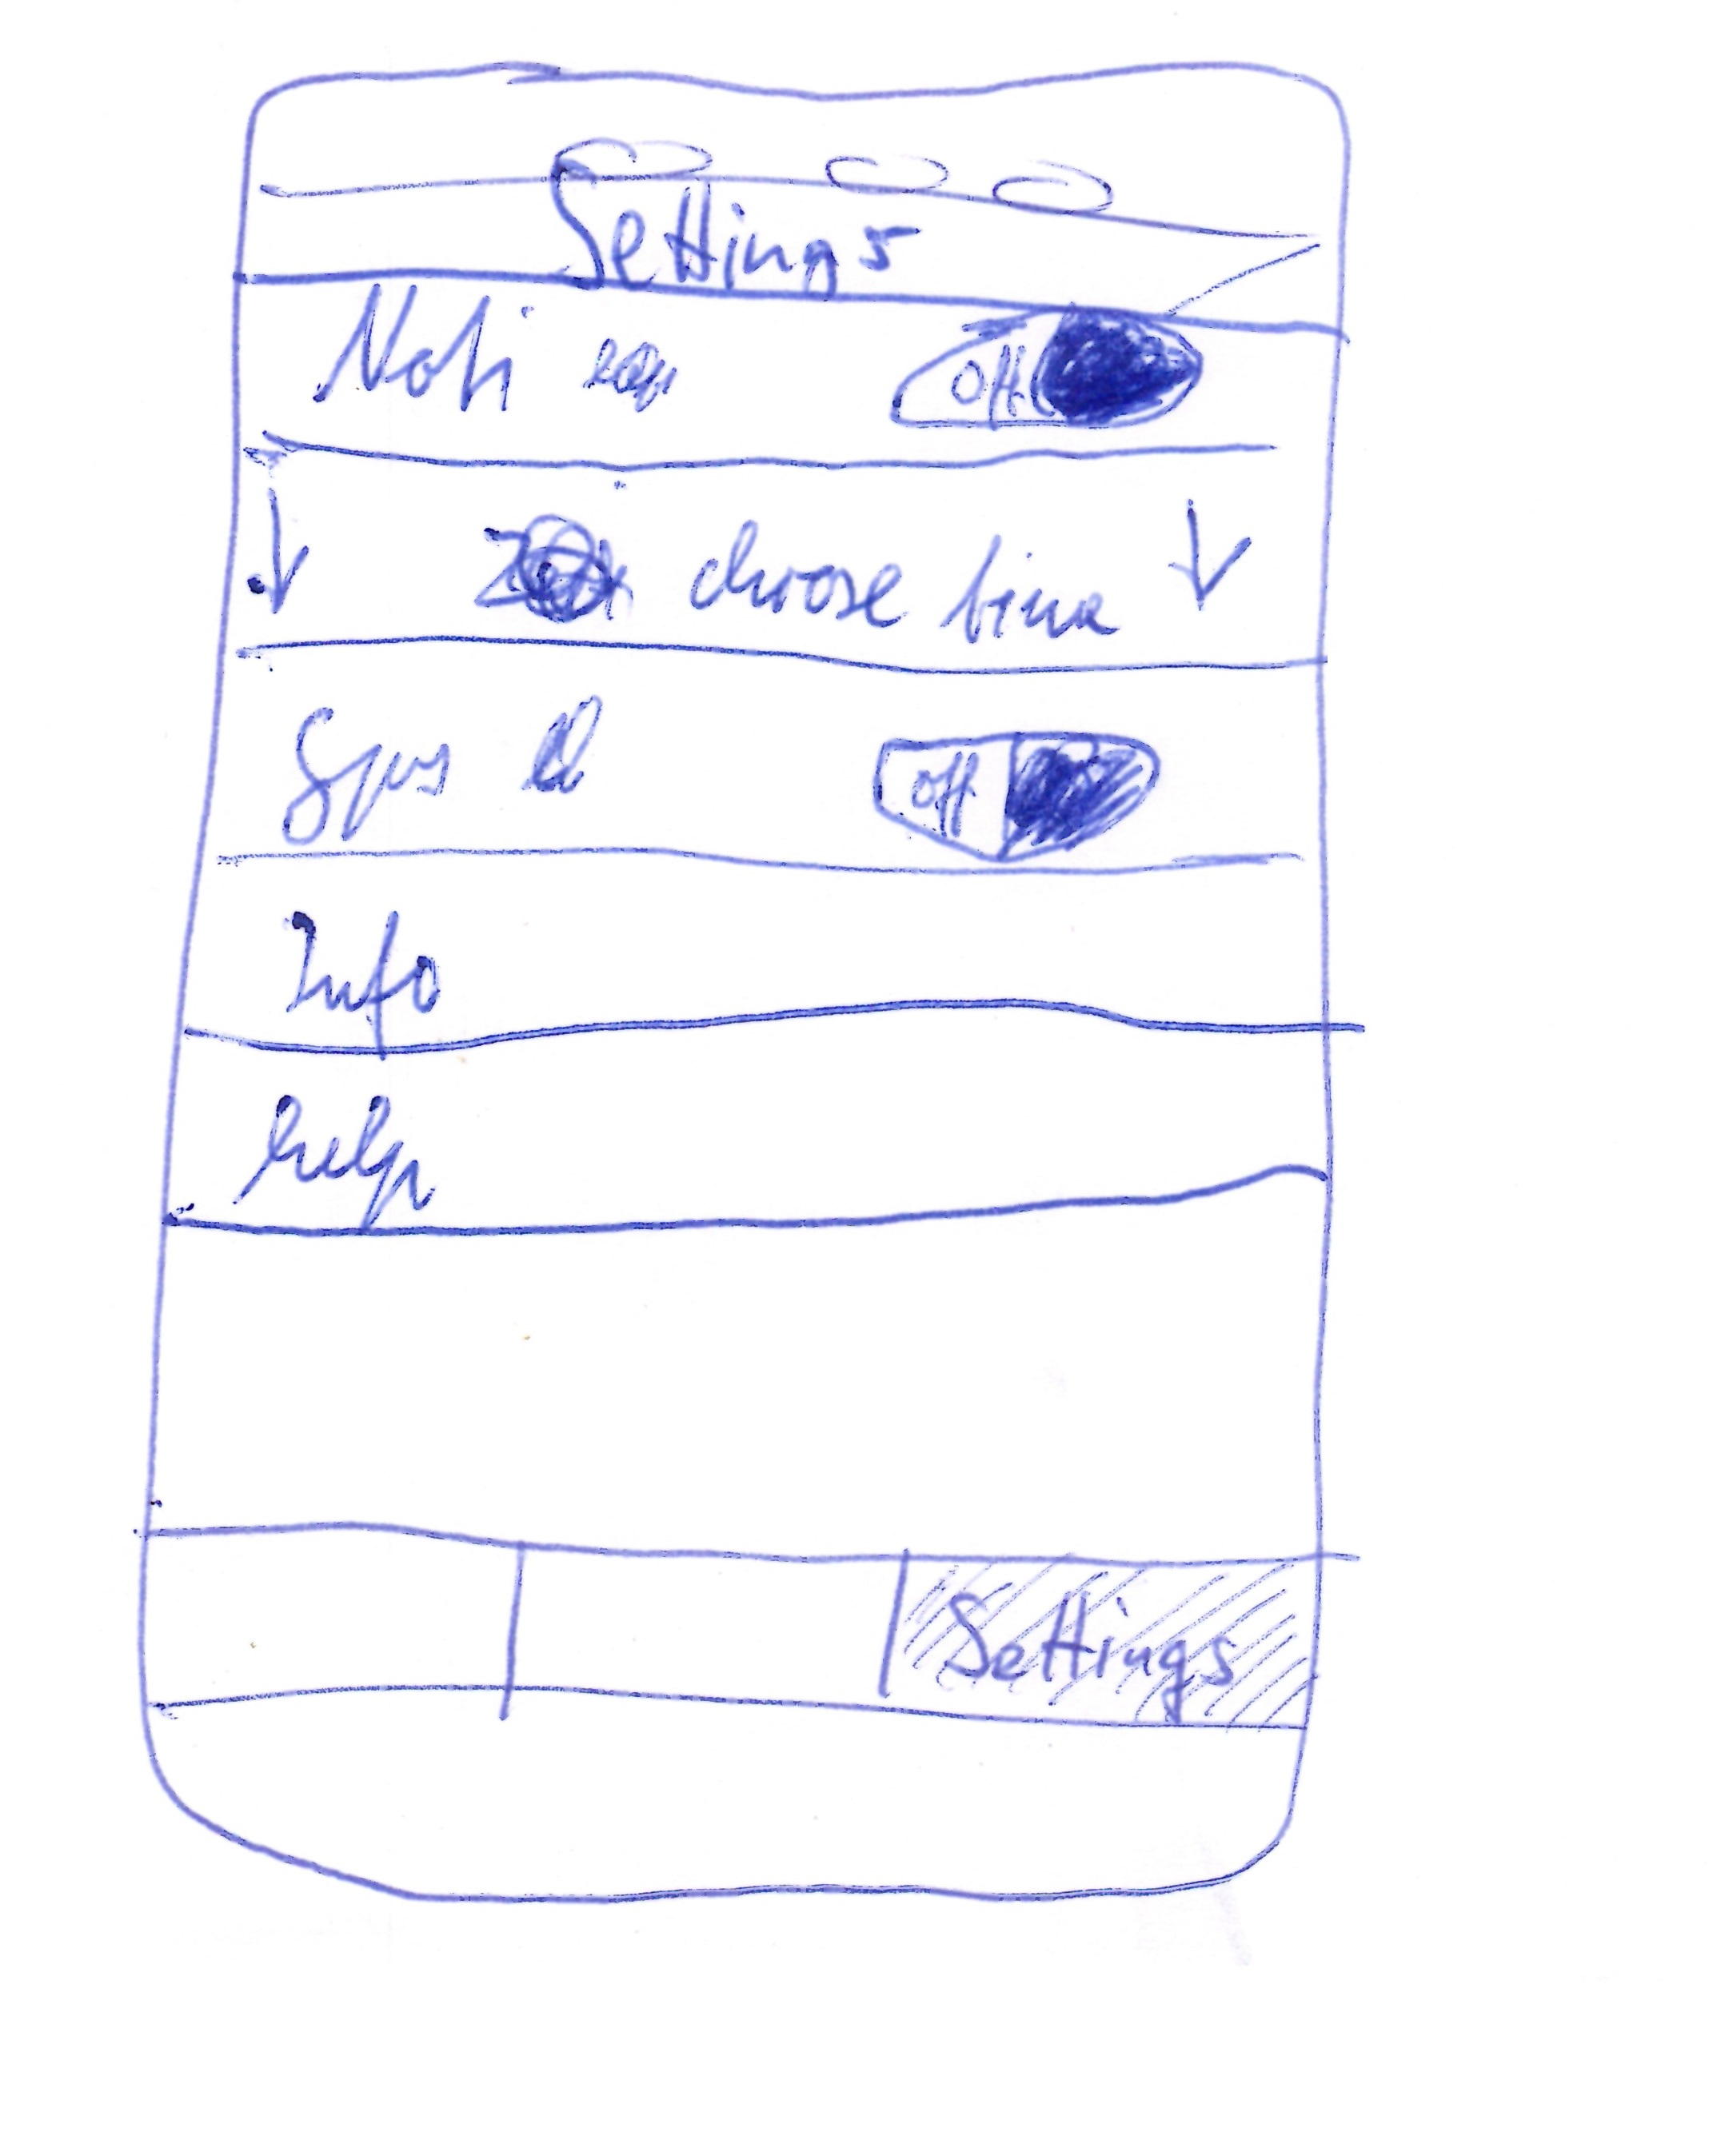
\includegraphics[scale=0.7]{settings} }
	\caption{Settings Screen}
	\label{settings}
\end{figure}


\section{Navigation Drawer Menü}
Der auch unter "Hamburger Menü" bekannte Navigation Drawer war einer der ersten Ideen für die App. Viele Funktionen später als Tab Bar bzw. als Icons in der oberen rechten Ecke umgesetzt wurden, sind diese Buttons an die genannten Stellen hin verschoben worden. Im Sinne der Anwenderfreundlichkeit wurde sich am Ende gegen den Navigation Drawer entschieden.
\begin{figure}[H]
	\centering
  \frame{ 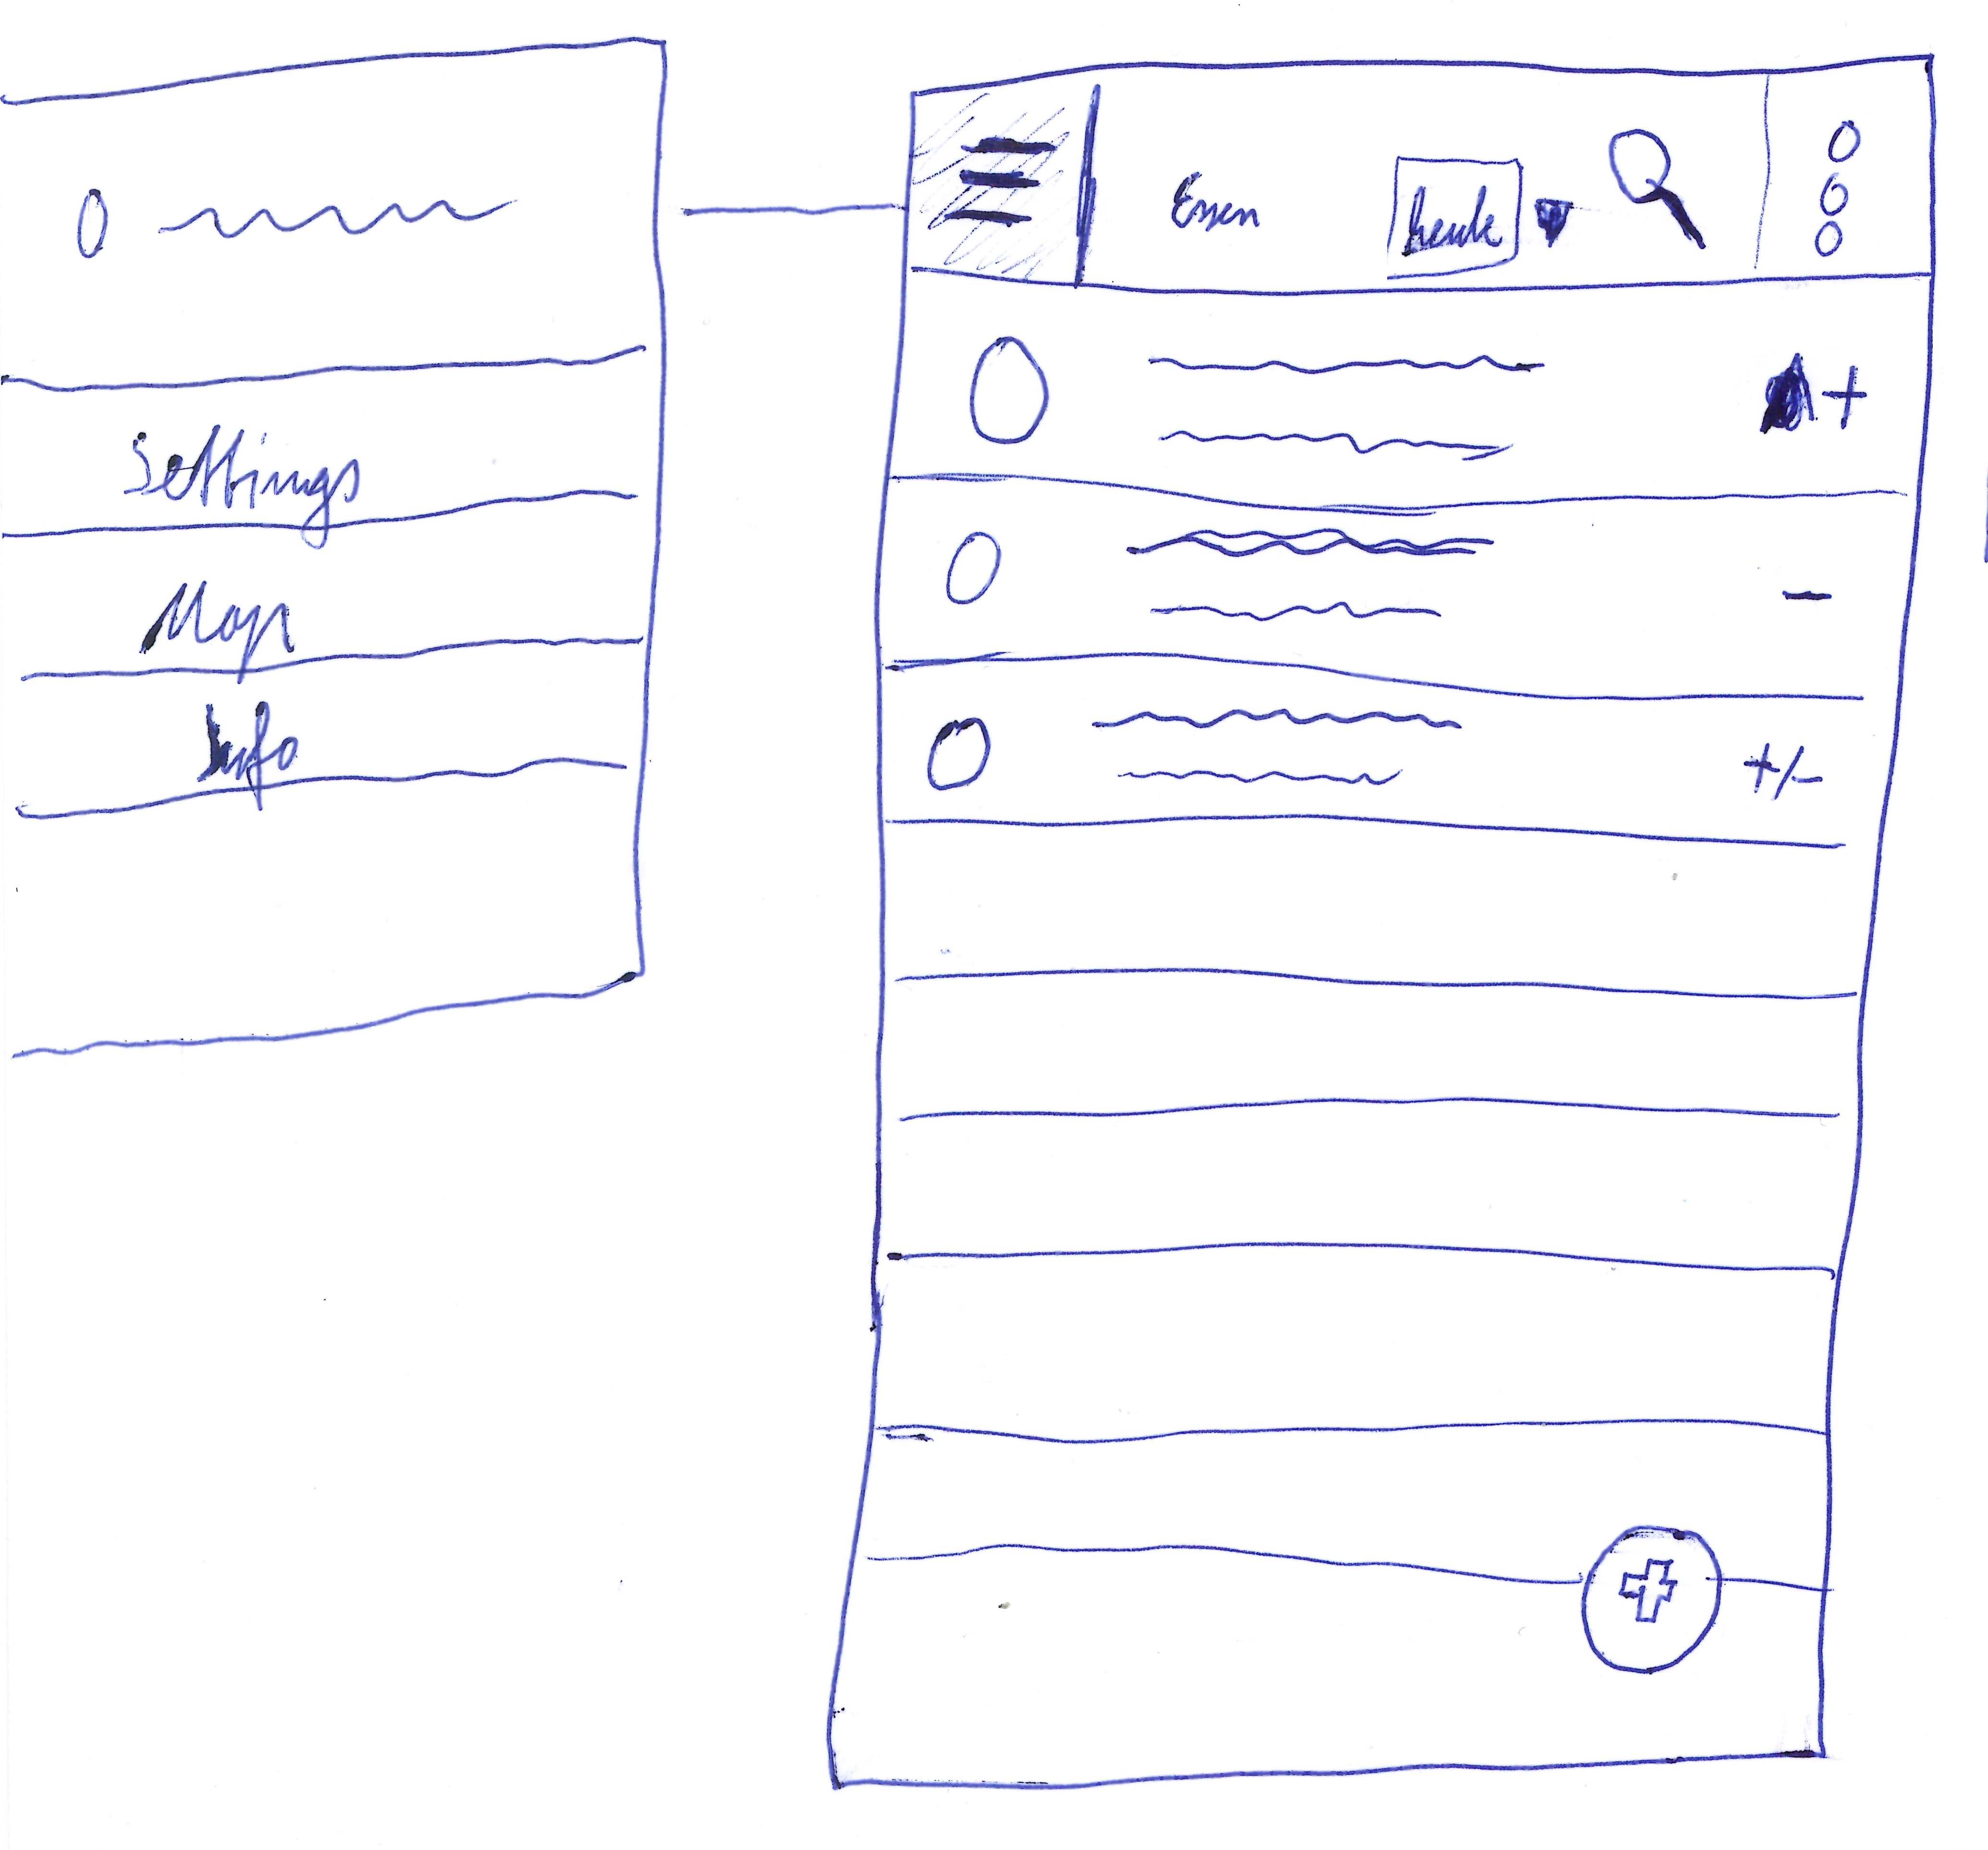
\includegraphics[scale=0.7]{main_burger} }
	\caption{Navigation Drawer Menü Screen}
	\label{main_burger}
\end{figure}


\section{Karten Screen}
Der Karten Screen zeigt eine Google Map. Darin repräsentieren Pins die Standorte an denen Essens Einträge hinzugefügt wurden.
\begin{figure}[H]
	\centering
  \frame{ 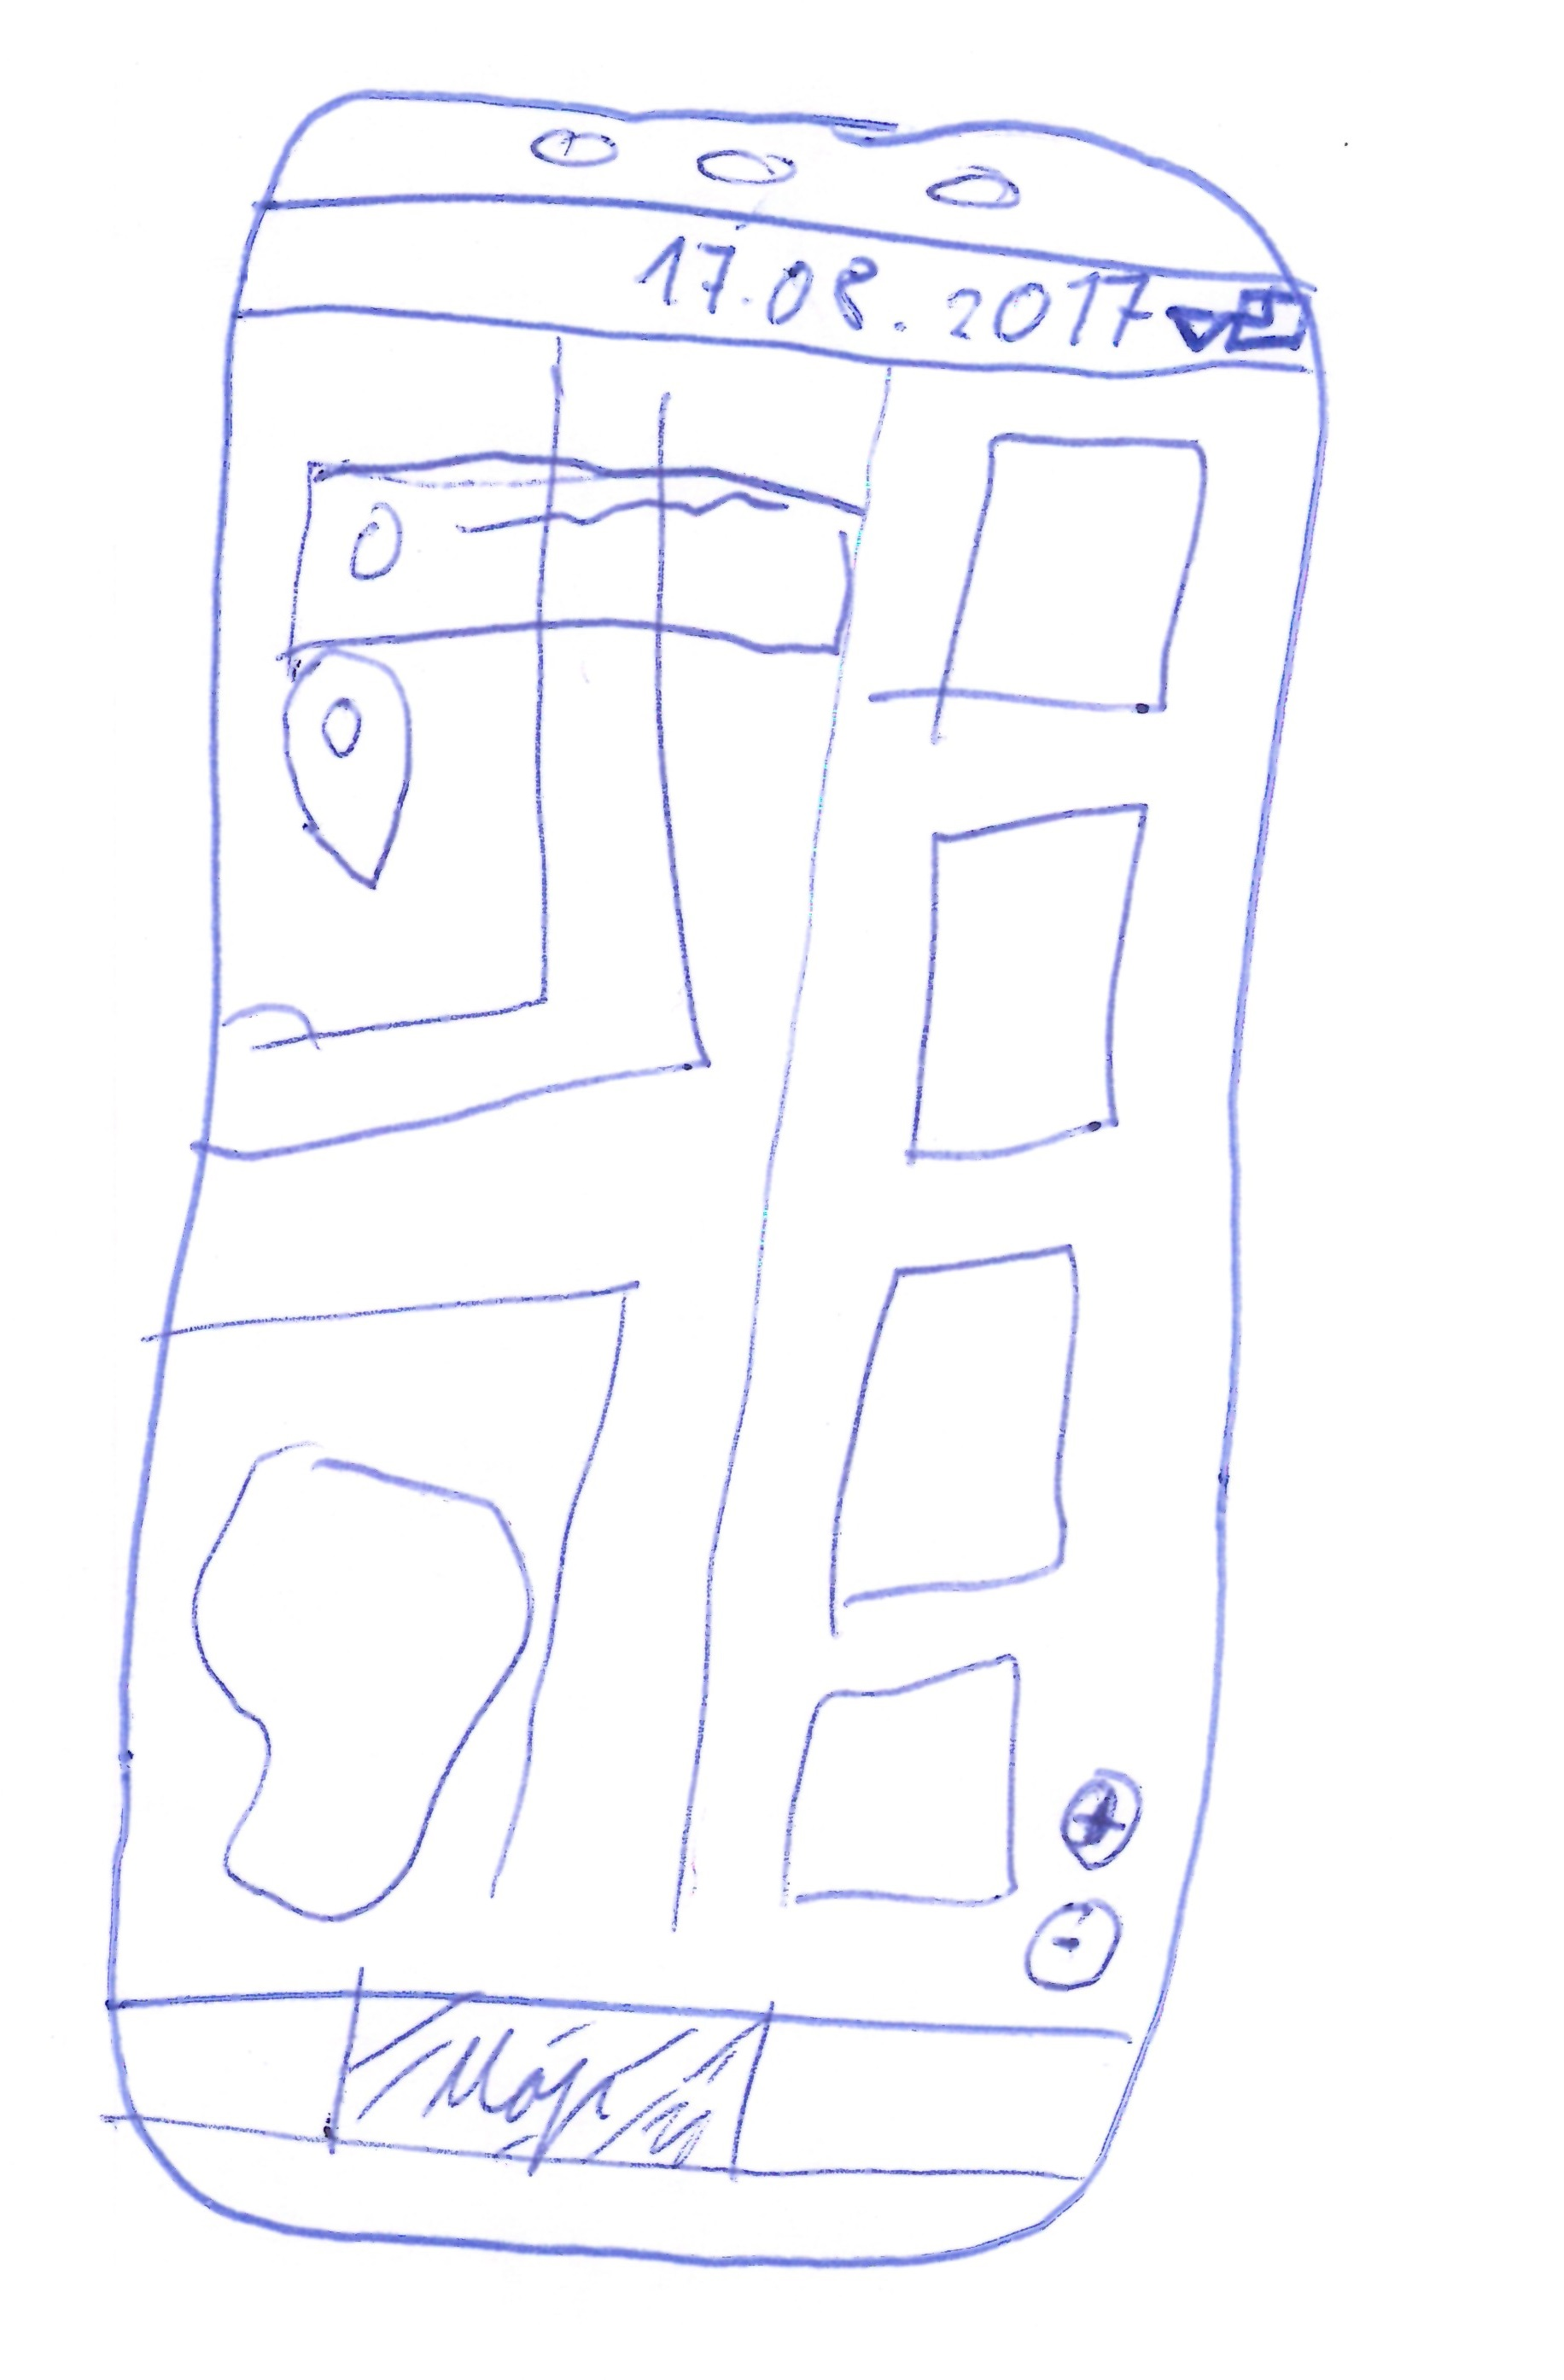
\includegraphics[scale=0.7]{map} }
	\caption{Karten Screen}
	\label{map}
\end{figure}




\newpage

\chapter{Umsetzung}
\section{Datenbank}
Für die Speicherung der Daten wurde sich für eine SQLite Datenbank entschieden. Das hat mehrere Vorteile. Zum einen lässt sich der Inhalt dieser Datenbank sehr einfach exportieren, um auf einem anderen Gerät wieder eingespielt werden zu können, zum anderen bietet eine Datenbankstruktur viele Möglichkeiten zur Datenanalyse mit schnellem Zugriff ohne wie bisher mit Files arbeiten zu müssen.

\subsection{Room}
Room wurde als Datenbank Abstraktionsschicht verwendet und bietet einfachen Datenbankzugriff ohne komplexe SQL Befehle.
\url{https://developer.android.com/topic/libraries/architecture/room.html}


\subsection{CSV Export}
Das Ausgabeformat CSV (Comma Separated Values) beschreibt den Aufbau einer Textdatei. Darin sind alle übergebenen Spaltennamen eingetragen. Die Reihenfolge der Spaltennamen gibt die Reihenfolge der Werte, die darunter aufgelistet sind wieder. Jeder Werteeintrag ist mit einem Return vom anderen getrennt.\\
Die App unterstützt den .CSV Export. Der Export wird als "FoodtrackerData.csv" File im Download Ordner gespeichert.
Dieser Ordner ist auf jedem Android Gerät einsehbar.



\section{Google Maps}
Für die Karte ist die Google Maps API eingesetzt worden. Darin wird für jeden Eintrag ein Pin in der Karte dargestellt.
Der API Key wurde dankensweise von Normen bereitgestellt.





\newpage

\chapter{Herausforderungen}
In jedem Projekt treten bei ansteigender Komplexität Probleme auf. Diese sind in diesem Abschnitt vermerkt.

\begin{itemize}
\item Aufwändige Integration von Dagger 2 die letztendlich verworfen werden musste. Mangelnde Dokumentation. Probleme beim Integrieren von bereits vorhandenen Projekten.
\end{itemize}

\newpage

\chapter{Lessons learned}
Dem Parkinsonschen Gesetz folgend wurde die Features während der vorhandenen Zeit umgesetzt. Da während der Appentwicklung die Stundenplan App der Hochschule betreut wurde, entstand gelegentlich ein Interessen- und Ressourcenkonflikt. Letztendlich wurden die Änderungen an der Schnittstelle leicht gewichtet behandelt, da diese einen Mehrwert für viele Hundert Studenten auf Android und iOS Seite mit sich brachten.


\newpage

\chapter{Weitere Arbeiten}
In diesem Projektabschnitt konnten alle gesteckten Ziele erreicht werden. Da solch ein junges Projekt noch viele Möglichkeiten beinhaltet Funktionen zu verbessern und neue Funktionen einzuführen werden hier mögliche Punkte zur Anregung aufgelistet. Da das Projekt als Open Source Projekt auf GitHub zur Verfügung steht, sind forks und pull pull requests willkommen. Da das Projekt somit der Öffentlichkeit übergeben wurde, besteht durchaus ein Interesse unsererseits die App weiter zu entwickeln.





\newpage


\listoffigures

\end{document}